%%%%%%%%%%%%%%%%%%%%%%%%%%%%%%%%%%%%%%%%%
% Journal Article
% LaTeX Template
% Version 2.0 (February 7, 2023)
%
% This template originates from:
% https://www.LaTeXTemplates.com
%
% Author:
% Vel (vel@latextemplates.com)
%
% License:
% CC BY-NC-SA 4.0 (https://creativecommons.org/licenses/by-nc-sa/4.0/)
%
% NOTE: The bibliography needs to be compiled using the biber engine.
%
%%%%%%%%%%%%%%%%%%%%%%%%%%%%%%%%%%%%%%%%%

%----------------------------------------------------------------------------------------
%	PACKAGES AND OTHER DOCUMENT CONFIGURATIONS
%----------------------------------------------------------------------------------------

\documentclass[
	a4paper, % Paper size, use either a4paper or letterpaper
	10pt, % Default font size, can also use 11pt or 12pt, although this is not recommended
	unnumberedsections, % Comment to enable section numbering
	twoside, % Two side traditional mode where headers and footers change between odd and even pages, comment this option to make them fixed
]{LTJournalArticle}

\addbibresource{article.bib} % BibLaTeX bibliography file

\runninghead{Battle of the Ledgers} % A shortened article title to appear in the running head, leave this command empty for no running head

% \footertext{\textit{Journal of Biological Sampling} (2024) 12:533-684} % Text to appear in the footer, leave this command empty for no footer text

\setcounter{page}{1} % The page number of the first page, set this to a higher number if the article is to be part of an issue or larger work

%----------------------------------------------------------------------------------------
%	TITLE SECTION
%----------------------------------------------------------------------------------------

\title{Battle of the Ledgers: \\ A Deep Dive into Blockchain and Graph} % Article title, use manual lines breaks (\\) to beautify the layout

% Authors are listed in a comma-separated list with superscript numbers indicating affiliations
% \thanks{} is used for any text that should be placed in a footnote on the first page, such as the corresponding author's email, journal acceptance dates, a copyright/license notice, keywords, etc
\author{%
	Samuel Polgar\thanks{Corresponding author: \href{mailto:spol2078@uni.sydney.edu.au}{spol2078@uni.sydney.edu.au}\\ \textbf{Published:} April 18, 2023}
}

% Full-width abstract
\renewcommand{\maketitlehookd}{%
	\begin{abstract}
		\noindent While Ethereum is a well-established blockchain platform that has recently transitioned to a proof-of-stake consensus mechanism, Hedera is a newer third-generation Distributed Ledger Technology (DLT) that uses a Directed Acyclic Graph (DAG). Both platforms have unique strengths and weaknesses when it comes to consensus, network incentives, and transaction processing. The report will examine these factors in detail, with a particular focus on the unique capabilities of each platform. By doing so, the report aims to provide insights that can help organizations make informed decisions when selecting a DLT for their needs.
	\end{abstract}
}

%----------------------------------------------------------------------------------------

\begin{document}

\maketitle % Output the title section

%----------------------------------------------------------------------------------------
%	ARTICLE CONTENTS
%----------------------------------------------------------------------------------------

\section{Introduction}

Blockchain technology has emerged as a promising solution to many of the limitations of trusted, centralized systems. With its decentralized and trustless nature, blockchain has the potential to revolutionize industries from finance to healthcare. Bitcoin was the first successful implementation of a distributed ledger, with Ethereum later introducing the Ethereum Virtual Machine (EVM), smart contracts, and trustless, decentralized applications. However, the limitations of early blockchains, such as scalability, the ability to process transactions and finality, the assurance that a transaction has successfully completed, have led to the development of newer technologies like Hedera Hashgraph. This report will compare and analyze the consensus mechanisms, providing insights into their strengths and weaknesses for potential use cases in the financial services industry.


%------------------------------------------------

\section{Problem Description}

Ethereum and other first-generation blockchains have successfully increased transparency, efficiency, and accessibility to financial services, attracting confident investors and resulting in over \$60B USD locked in DeFi, although it has been as high as over \$200B. However, limitations arising from its consensus mechanism (PoS) such as transaction per second speed, probabilistic finality, and non-fair ordering constrain future success.

Hedera Hashgraph, a third-generation DLT, builds upon the promise of DeFi by addressing some of the shortcomings of its predecessors. As a Directed Acyclic Graph (DAG), Hedera Hashgraph and its unique consensus mechanism—Gossip about Gossip and Virtual Voting (GaGVV)—resolve these issues by offering incredible transaction per second speed, fast deterministic finality, and fair transaction ordering. These advancements position DeFi for continued expansion and growth in the financial services industry.

\section{Distributed Ledger Comparison}

A Blockchain and Directed Acyclic Graph (DAG) are two different types of DLT’s – both record transactions and maintain a shared database of transactions \cite{lashkari_comprehensive_2021}.
As the represented in Figure 1. A blockchain is a linear set of connected blocks, like a chain, each block contains a set of transactions that have been validated to be true by network consensus and are linearly linked to future blocks. In contrast, a DAG is graph structure where the events (similar to blocks) can be connected to multiple other events.
\begin{figure}[h]
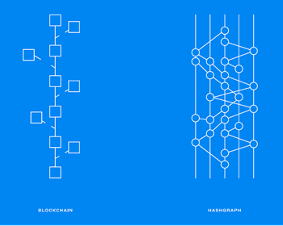
\includegraphics[width=8cm]{blockchainAndGraph.png}
\caption{Figure 1 Depiction of a Blockchain and Graph}
\end{figure}

Ethereum’s Blockchain and Hedera’s Graph differ in the way they store information, including the current state of the network and transaction history \cite{b_anupama_analysis_2022}. Ethereum nodes hold a copy of all transactions since the beginning of the blockchain, and each new block contains multiple transactions that a validator node must verify before broadcasting aka Gossiping to the network for consensus. In contrast, Hedera's nodes can perform this operation asynchronously, allowing multiple blocks to be processed simultaneously with a consistent state. Unlike Ethereum, Hedera's nodes only store the current state of the network, freeing up computing resources for transaction processing and consensus. Separate nodes can be created for historical transaction storage.

\section{Consensus Comparison}

\subsection{Ethereum}

Ethereum uses Proof of Stake (PoS) for consensus, in summary \cite{buterin_casper_2017,vitalik_buterin_incentives_2019,o_moindrot_proof_2017}\begin{enumerate}
\item Validator nodes stake 32 Ethereum (the native currency) for the opportunity to validate a block
\item The protocol randomly selects a node from the network of over 9600 nodes to participate in block validation
\item The selected node becomes the leader, choosing which transactions to include in the block and proposing it to the network
\item The leader selects transactions from the mempool where all Ethereum transactions are stored before being processed. They typically prioritize transactions with the highest fee, as the validator will earn more Ethere by validating the block
\item The leader risks losing some or all of their staked Ether if they attempt to produce a malicious block that is detected by the network
\item The block is then gossiped out to the network
\end{enumerate}

\subsection{Hedera Hashgraph}
Hedera Hashgraph uses a weighted Proof of Stake (PoS) consensus mechanism, as outlined below \cite{baird_swirlds_nodate}:
\begin{enumerate}
\item Validator nodes stake HBAR (the native currency) for the opportunity to validate events
\item The protocol selects nodes, based on the weight of HBAR they stake
\item Hashgraph is leaderless – once a transaction is sent to a node and the node validates the transaction, it then gossips the event to other nodes on the network
\item In parallel, other network nodes perform the same task, validating transactions and gossiping events
\item Hashgraph nodes immediately validate the transaction and send it out to the network, it doesn’t pick transactions from a mempool
\item Blocks are continuously gossiped to the network to ensure every node knows every event
\item Nodes use the virtual voting algorithm to validate transactions and place transactions in fair ordering based on the event timestamps and voting algorithm
\end{enumerate}

\section{Key Defining Attributes}


\begin{longtable}{|l|l|l|}
\hline
Property               & Ethereum   & Hedera Hashgraph \\ \hline
\endfirsthead
%
\endhead
%
Consensus Algorithm &  PoS & GaGVV \\ \hline
\begin{tabular}[c]{@{}l@{}}Avg. Transaction \\    energy\end{tabular} &
  0.03 kWh &
  0.0001 kWh \\ \hline
Leader / Leaderless    & Leader     & Leaderless       \\ \hline
Finality               & 15 Minutes & 2 – 3 seconds    \\ \hline
Fair transaction order & No         & Yes              \\ \hline
Safety (fork risk)     & Low        & None             \\ \hline
DDoS risk              & Low        & Extremely Low    \\ \hline
Node Memory Use        & Medium     & Low              \\ \hline
\caption{Comparing attributes between Ethereum and Hedera}
\label{tab:key-points-comparison}\\
\end{longtable}

\begin{figure*}
	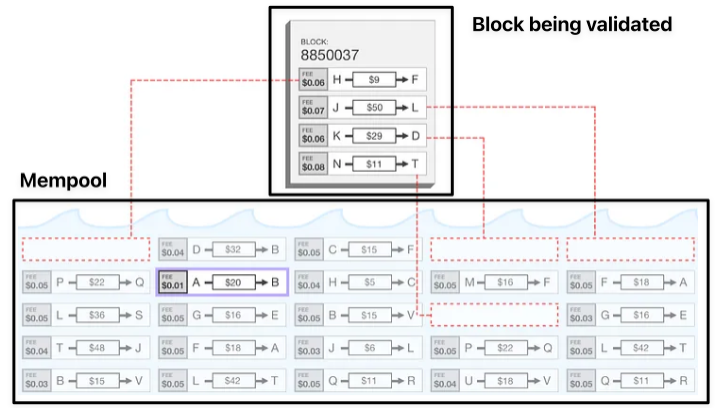
\includegraphics[width=\linewidth]{mempool.png}
	\caption{Diagram of the mempool}
 \label{fig:mempool}
\end{figure*}

\subsection{The Mempool}
The mempool (memory pool) is a temporary storage area for unconfirmed transactions awaiting validation within a network. The mempool impacts transaction throughput speed and fee dynamics. Users conducting transactions on the blockchain are charged a fee, and they can effectively prioritize their transactions by increasing the fee they are willing to pay. Mempools provide validators the opportunity to earn additional fees, thereby promoting greater decentralization with more validator nodes. However, this approach has several downsides:
\begin{itemize}
    \item Transaction ordering: Transactions with higher fees can leapfrog older transactions, resulting in unfair ordering, as viewed in Figure 3. This poses a risk for financial and legal services that rely on fair and chronological processing
    \item Network congestion: Mempools can create bottlenecks during periods of high transaction volume, leading to delays and increased fees
    \item Uncertain transactions: Transactions with low fees (as determined by the user) may not be processed, creating uncertainty for users regarding their transaction status 
    \item Transaction front-running: Adversaries may monitor the mempool with algorithms and bots to "outsmart" other transactions by strategically placing their own transactions with higher fees
\end{itemize}
Referencing a figure using its label: Figure \ref{fig:mempool}.
Hedera Hashgraph, in contrast, does not use a mempool. Instead, validator nodes immediately validate transactions and disseminate the information through the network using the gossip protocol. This approach avoids the aforementioned issues, resulting in a more efficient and fair transaction processing system.

\subsection{Byzantine Fault Tolerance}
Byzantine Fault Tolerance (BFT) is a property of distributed systems akin to a measurement of their ability to tolerate failures or malicious behavior by network nodes or adversaries \cite{lamport_byzantine_2019}. BFT guarantees that a distributed system will continue to operate and reach consensus despite a number of attacks such as DDOS, malicious or failing nodes.
Ethereum is Byzantine Fault Tolerant (BFT) whereas Hedera Hashgraph is asynchronous Byzantine Fault Tolerant (aBFT) – ABFT is the strongest security guarantee for a distributed system \cite{james_experimental_2019}. Differences in Hashgraph’s architecture and consensus mechanism enables ABFT

\subsection{Leader vs Leaderless}
Ethereum's consensus mechanism is leader-based, where a randomly selected node becomes the leader responsible for proposing new blocks. Hedera Hashgraph, in contrast, is leaderless, which means every node on the network has equal responsibility for validating and gossiping transactions. This difference impacts the scalability, performance, and security of both platforms.

\subsection{Finality}
Finality is the point at which a transaction is considered immutable \cite{pan_plume_2021}. Ethereum’s PoS provides probabilistic finality. The longer the Ethereum chain is, the less likely the transaction is change. Hedera Hashgraph provides fast, deterministic finality within seconds. Determinisitic finality is important for many industries, it’s important in law as the law doesn’t cater for probabilistic finality in cases of ownership and transactions.

\subsection{Fair Transaction Ordering}
Ethereum’s validators select transactions from the Ethereum Mempool, therefore, transactions are not validated and commited to chain in the order they’re received. This can cause issues with ledgers used for enterprise use today, for example, an immutable ledger for timestamped interactions, or transaction processing times. Hedera’s Hashgraph provides fair transaction ordering \cite{gross_co-founder_nodate}by removing the need for a mempool and ordering transactions based on timestamps and the virtual voting algorithm.

\subsection{Transaction Throughput}
Ethereum 1.0 recently upgraded to Ethereum 2.0, the current transaction throughput is not yet thoroughly tested – the popularity of layer-2 rollups and sidechains increase the number of transaction settlements that Ethereum can process. Ethereum 1.0 could process 15 – 30 transacts per second while Ethereum 2.0 (including sidechains and rollups) may process 3000 per second (including offchain computation, onchain settlement). Currently, Hedera Hashgraph can process 10,000 transactions per second, with the potential for greater throughput \cite{james_experimental_2019}. 

\section{Evaluation for the Financial Services Industry}
Ethereum’s success in Decentralized Finance (DeFi) has proven its ability as a robust financial infrastructure, tested with over \$200Billion USD locked in December 2021.
Despite the initial success being used as financial infrastructure in Decentralized Finance (DeFi), first-generation implementations like Ethereum currently fall short in meeting the specific requirements of an enterprise financial infrastructure. 

Hedera Hashgraph's unique approach to distributed ledger technology, with its resource-efficient storage, leaderless consensus, and asynchronous Byzantine Fault Tolerance (aBFT), offers promising potential for use in financial services. Hedera's consensus mechanism ensures robust security, essential for maintaining trust in the financial sector. The platform's fast, deterministic finality enables clear records of ownership and transaction history, meeting legal and regulatory requirements. Additionally, Hedera's fair transaction ordering promotes impartiality and transparency in transaction processing \cite{baird_swirlds_nodate}.
Hedera's high transaction throughput, capable of processing 10,000 transactions per second, surpasses Ethereum's capabilities, making it suitable for large-scale, real-time financial applications. However, when considering Hedera for banking systems, it is crucial to account for regulatory compliance, adoption, and integration with existing infrastructure. Overall, Hedera Hashgraph presents a strong case for adoption in the banking industry, given its efficiency, security, and scalability features.

\printbibliography % Output the bibliography

%----------------------------------------------------------------------------------------

\end{document}

\bibliographystyle{plain}
\bibliography{bib2}
